\section{Forward Tracking System}
\label{overview}

The CLAS12 forward detector is constructed around a toroidal magnet consisting of six 
iron-free superconducting coils.  The particle detection system consists of drift 
chambers to determine charged-particle trajectories, {\v C}erenkov detectors 
for electron/pion separation, scintillation counters for flight-time 
measurements, and calorimeters to identify electrons and high-energy neutral 
particles.  An overview of the CLAS12 subsystems and geometry may be found in the 
CLAS12 Overview paper ~\cite{clas12-overview} in this volume.  A schematic view of the 
torus magnet with drift chambers
attached is shown in Fig.~\ref{chambers-and-torus}.   The drift chambers are 
triangular boxes attached to the magnet cryostat by ``rod and ball and socket'' sets.  
This assembly of magnet and chambers is referred to as the ``forward tracker''. 

The forward tracker can detect charged particles emerging from the target with
momenta greater than 200~MeV/c over a polar angular range from roughly 5$^{\circ}$ to 
40$^{\circ}$.  Because the coils of the torus magnet represent a ``dead area''
in which we cannot detect charged particles, we designed the chamber endplates
and attached electronics to be as thin as possible.  The resulting azimuthal
coverage varied from 50\% of 2$\pi$ at 5$^{\circ}$ to 80\% of 2$\pi$ at 40$^{\circ}$.


%%%%%%%%%%%%%%%%%%%%%% Figure : CLAS 3D Picture %%%%%%%%%%%%%%%%%%%%%%%%%%%%%%%
\begin{figure}[htbp]
\vspace{10cm}
\begin{picture}(25,25)
\put(-10,10)
{\hbox{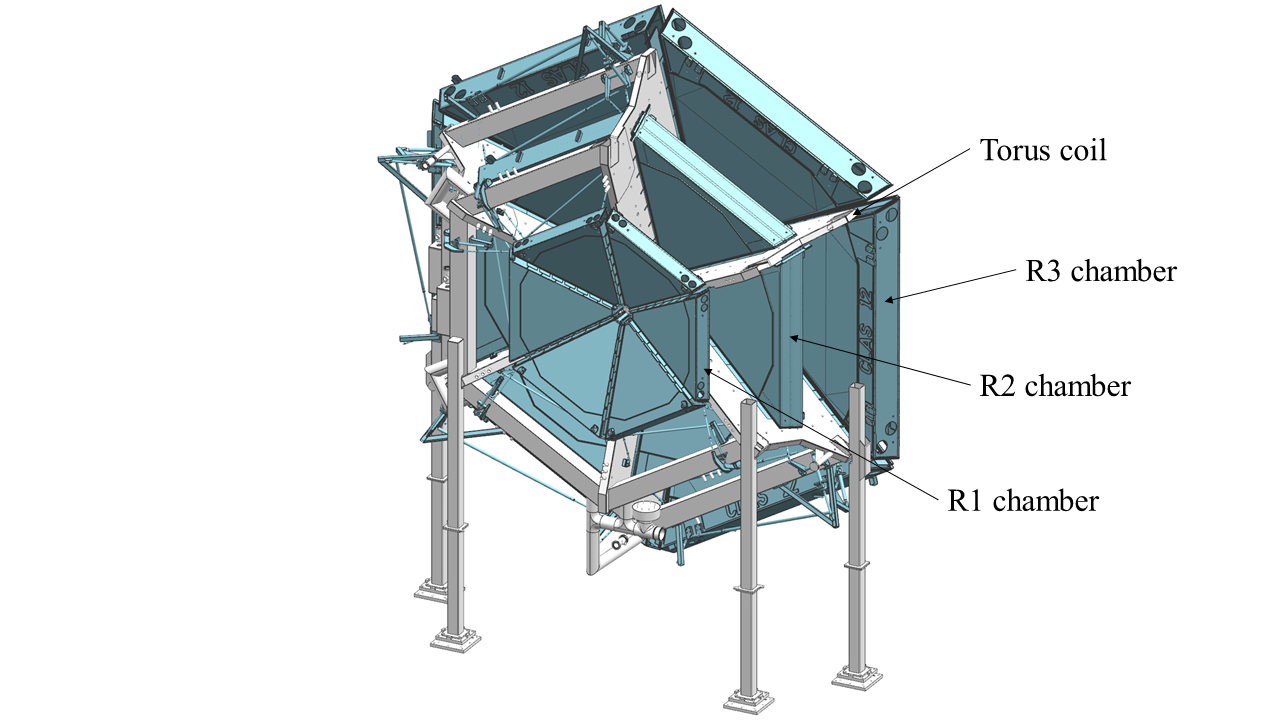
\includegraphics[width=1.\textwidth,natwidth=610,natheight=642]{img/chambers-and-torus.png}}}
\end{picture}
\caption{\small{A sketch of the torus magnet with drift chambers attached.
Note that cable runs and gas lines have been removed for clarity.  The largest
(R3) chambers are approximately equilateral triangular solids with 4 m long sides
and 0.8 m depth.}}
\label{chambers-and-torus}
\end{figure}
%%%%%%%%%%%%%%%%%%%%%%%%%%%%%%%%%%%%%%%%%%%%%%%%%%%%%%%%%%%%%%%%%%%%%%%%%%%




















































